%%%%%%%%%%%%%%%%%%%%%%%%%%%%%%%%%%%%%%%%%%%%%%%%%%%%%%%%%%%%%%%%%%%%%%%%%%%%%%%

\section*{\large Exercício 8 - Global Wavelet Spectrum}
\addcontentsline{toc}{chapter}{\protect\numberline{}\large Exercício 8}%

Os resultados deste exercício se encontram na pasta \textbf{Exercise8}. Abaixo está a análise para a série de novos casos da Covid19 para o Brasil, de 30 de março a 5 de junho. Foi utilizado o pacode do Python waipy.

Os plots das ondeletas mãe Morlet e DoG (Derivative of Gaussian) indicam que a melhor escolha é a DoG, pois ela foi capaz de captar os períodos do sinal dentro do cone de influência, com um pico bem pronunciado no wavelet spectrum (Figura 8.2.1). Por outro lado, a ondeleta Morlet não foi capaz de apresentar o pico dentro do cone de influência (Figura 8.1.1).

\subsection*{8.1}
\addcontentsline{toc}{section}{\protect\numberline{} 8.1}%

Resultado da aplicação do pacote waipy com a wavelet mãe Morlet, aplicada sobre a série da Covid19 (novos casos diários) para o Brasil. O período do sinal não é bem captado pela ondeleta: o pico do espectro wavelet - em azul à direita - está fora do cone de influência. 

\begin{figure}[ht!]
	%\caption{Série e histogramas.}
	\vspace{0mm}	% acrescentar o espaçamento vertical apropriado entre o título e a borda superior da figura
	\begin{center}
		\resizebox{16cm}{!}{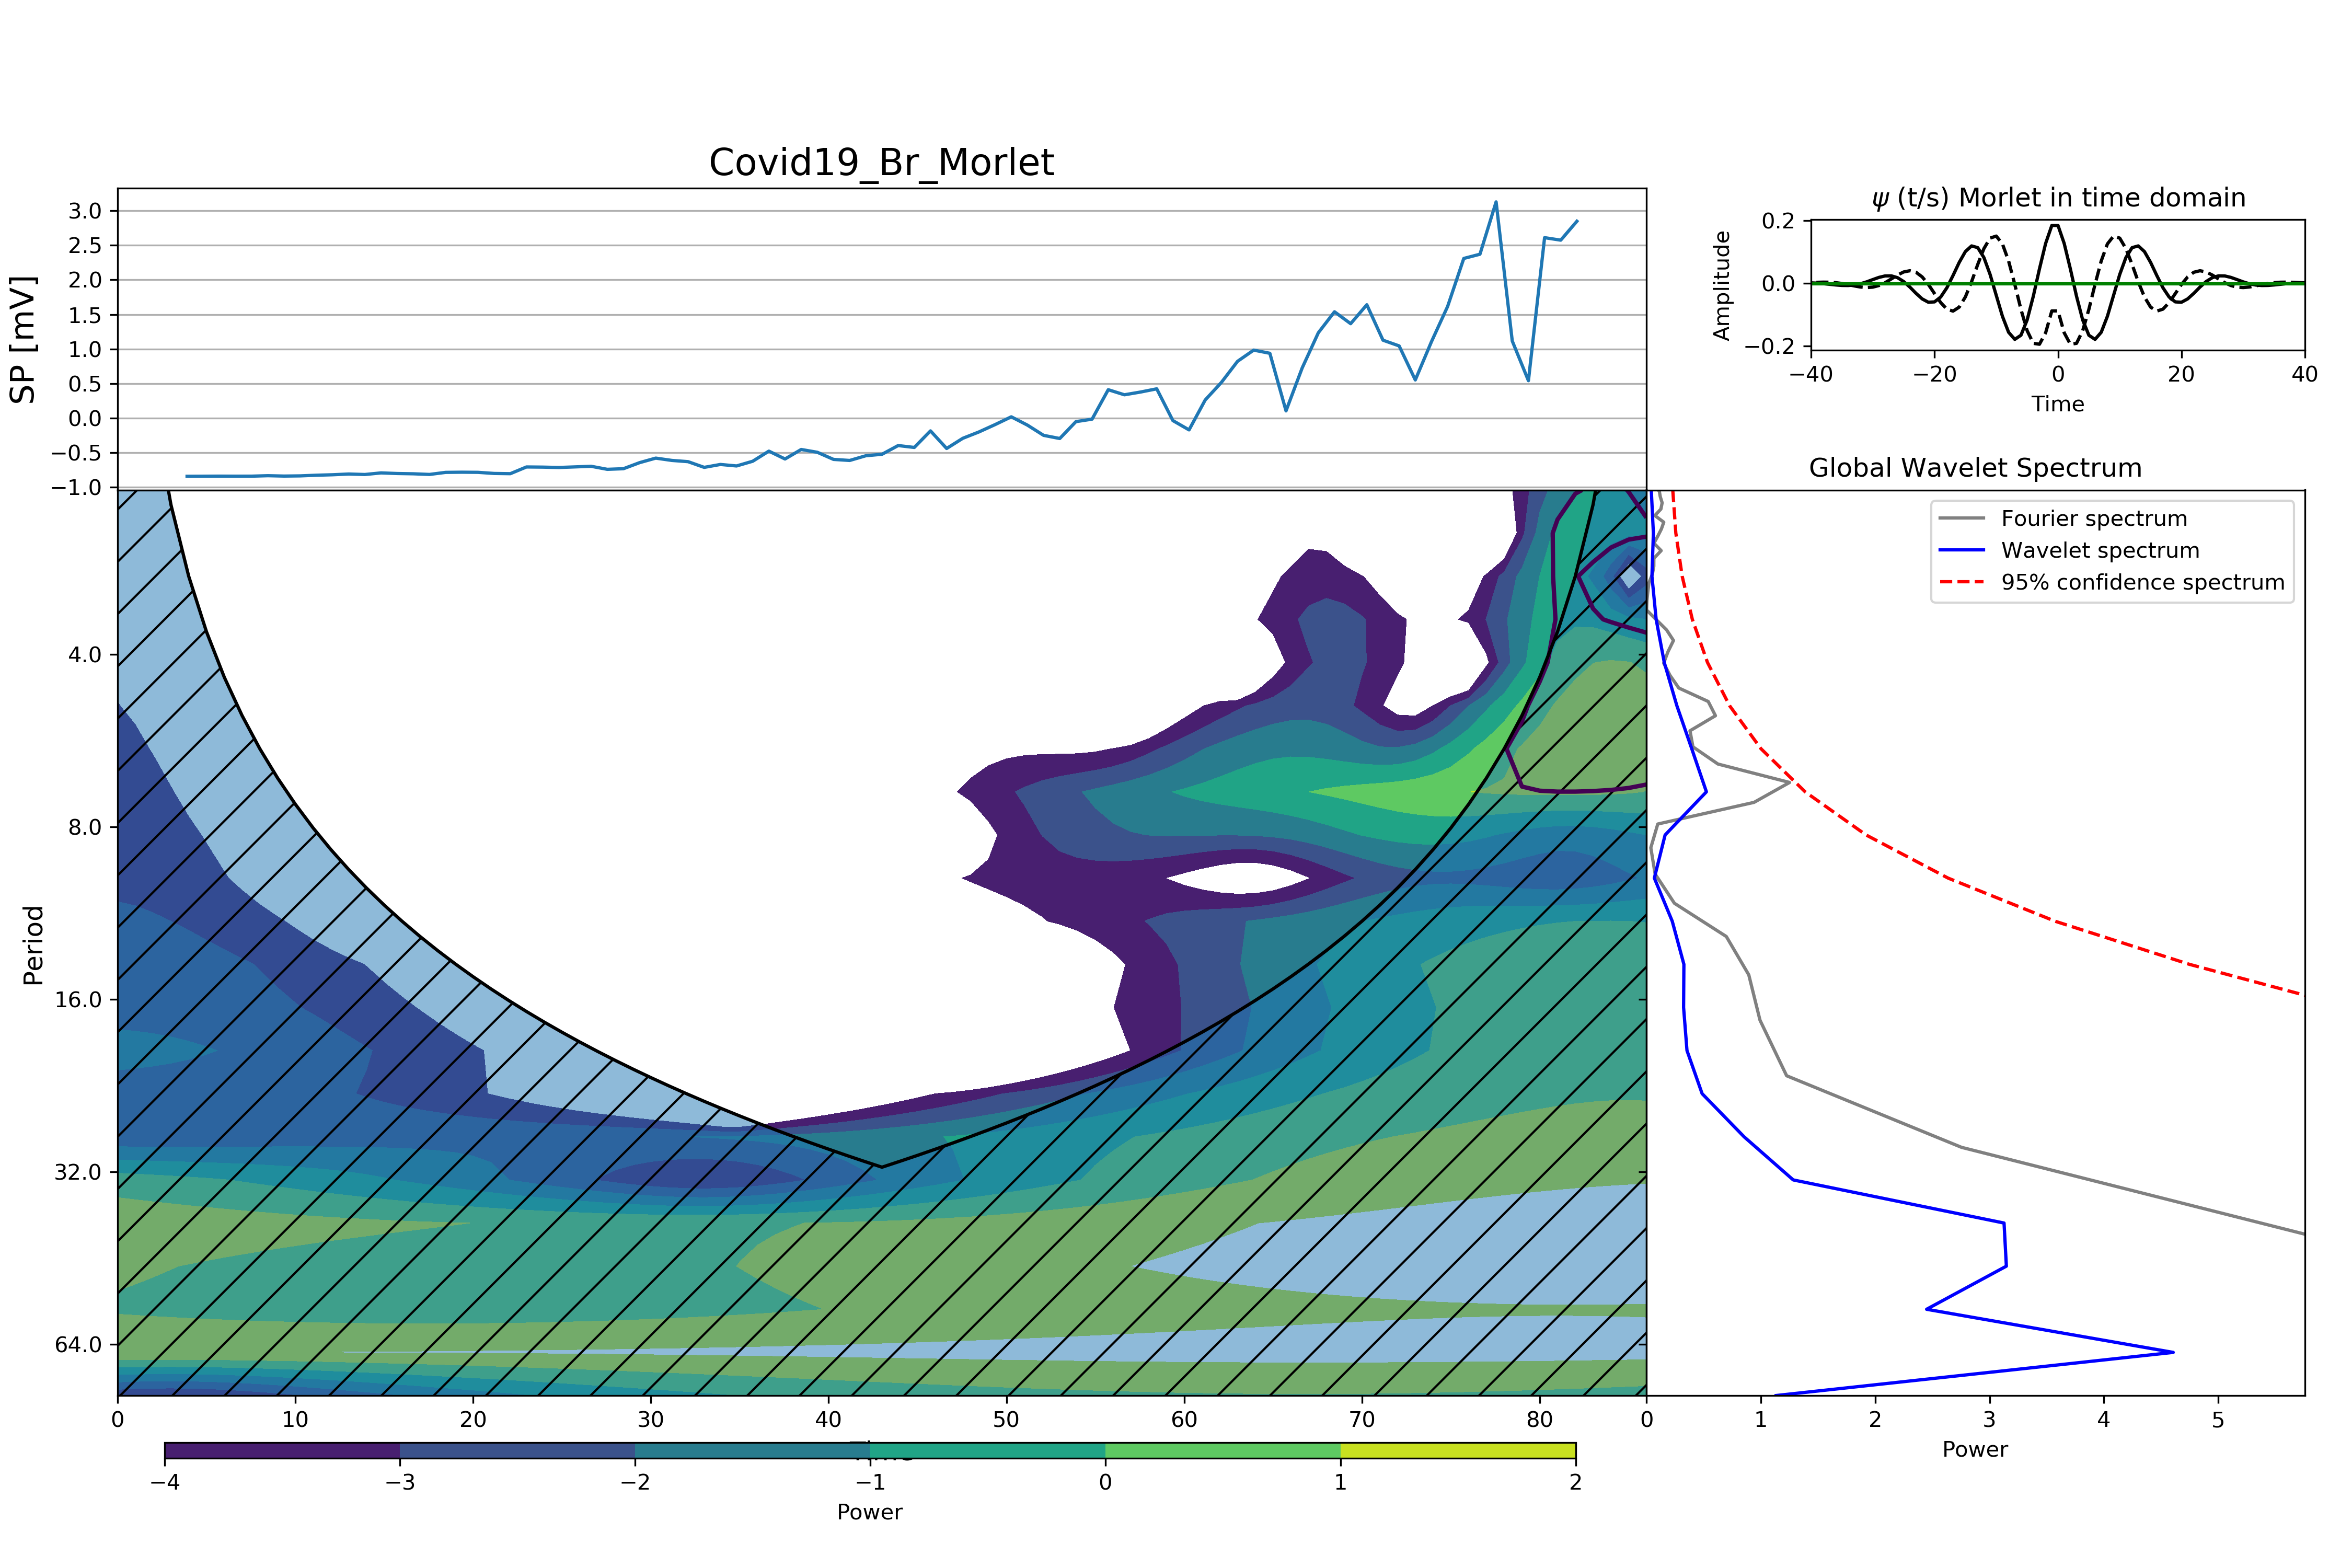
\includegraphics{Figuras/ex8/Covid19_Br_Morlet.png}}		
	\end{center}
	\vspace{-2mm}	% acrescentar o espaçamento vertical apropriado entre a borda inferior da figura e a legenda ou a fonte quando não há legenda (o valor pode ser negativo para subir)
	\legenda{Figura 8.1.1: Global Wavelet Spectrum da série de dados da Covid19 do Brasil com a ondeleta mãe Morlet.}	% legenda - para deixar sem legenda usar comando \legenda{} (nunca deve-se comentar o comando \legenda)
	\label{ex8_fig1}
	%\FONTE{}	% fonte consultada (elemento obrigatório, mesmo que seja produção do próprio autor)
\end{figure}

\clearpage
\subsection*{8.2}
\addcontentsline{toc}{section}{\protect\numberline{} 8.2}%

Resultado da aplicação do waipy com a wavelet mãe DoG, aplicada sobre a série da Covid19 (novos casos diários) para o Brasil. Parte do pico do espectro wavelet - em azul à direita - está dentro do cone de influência. 

\begin{figure}[ht!]
	%\caption{Série e histogramas.}
	\vspace{0mm}	% acrescentar o espaçamento vertical apropriado entre o título e a borda superior da figura
	\begin{center}
		\resizebox{16cm}{!}{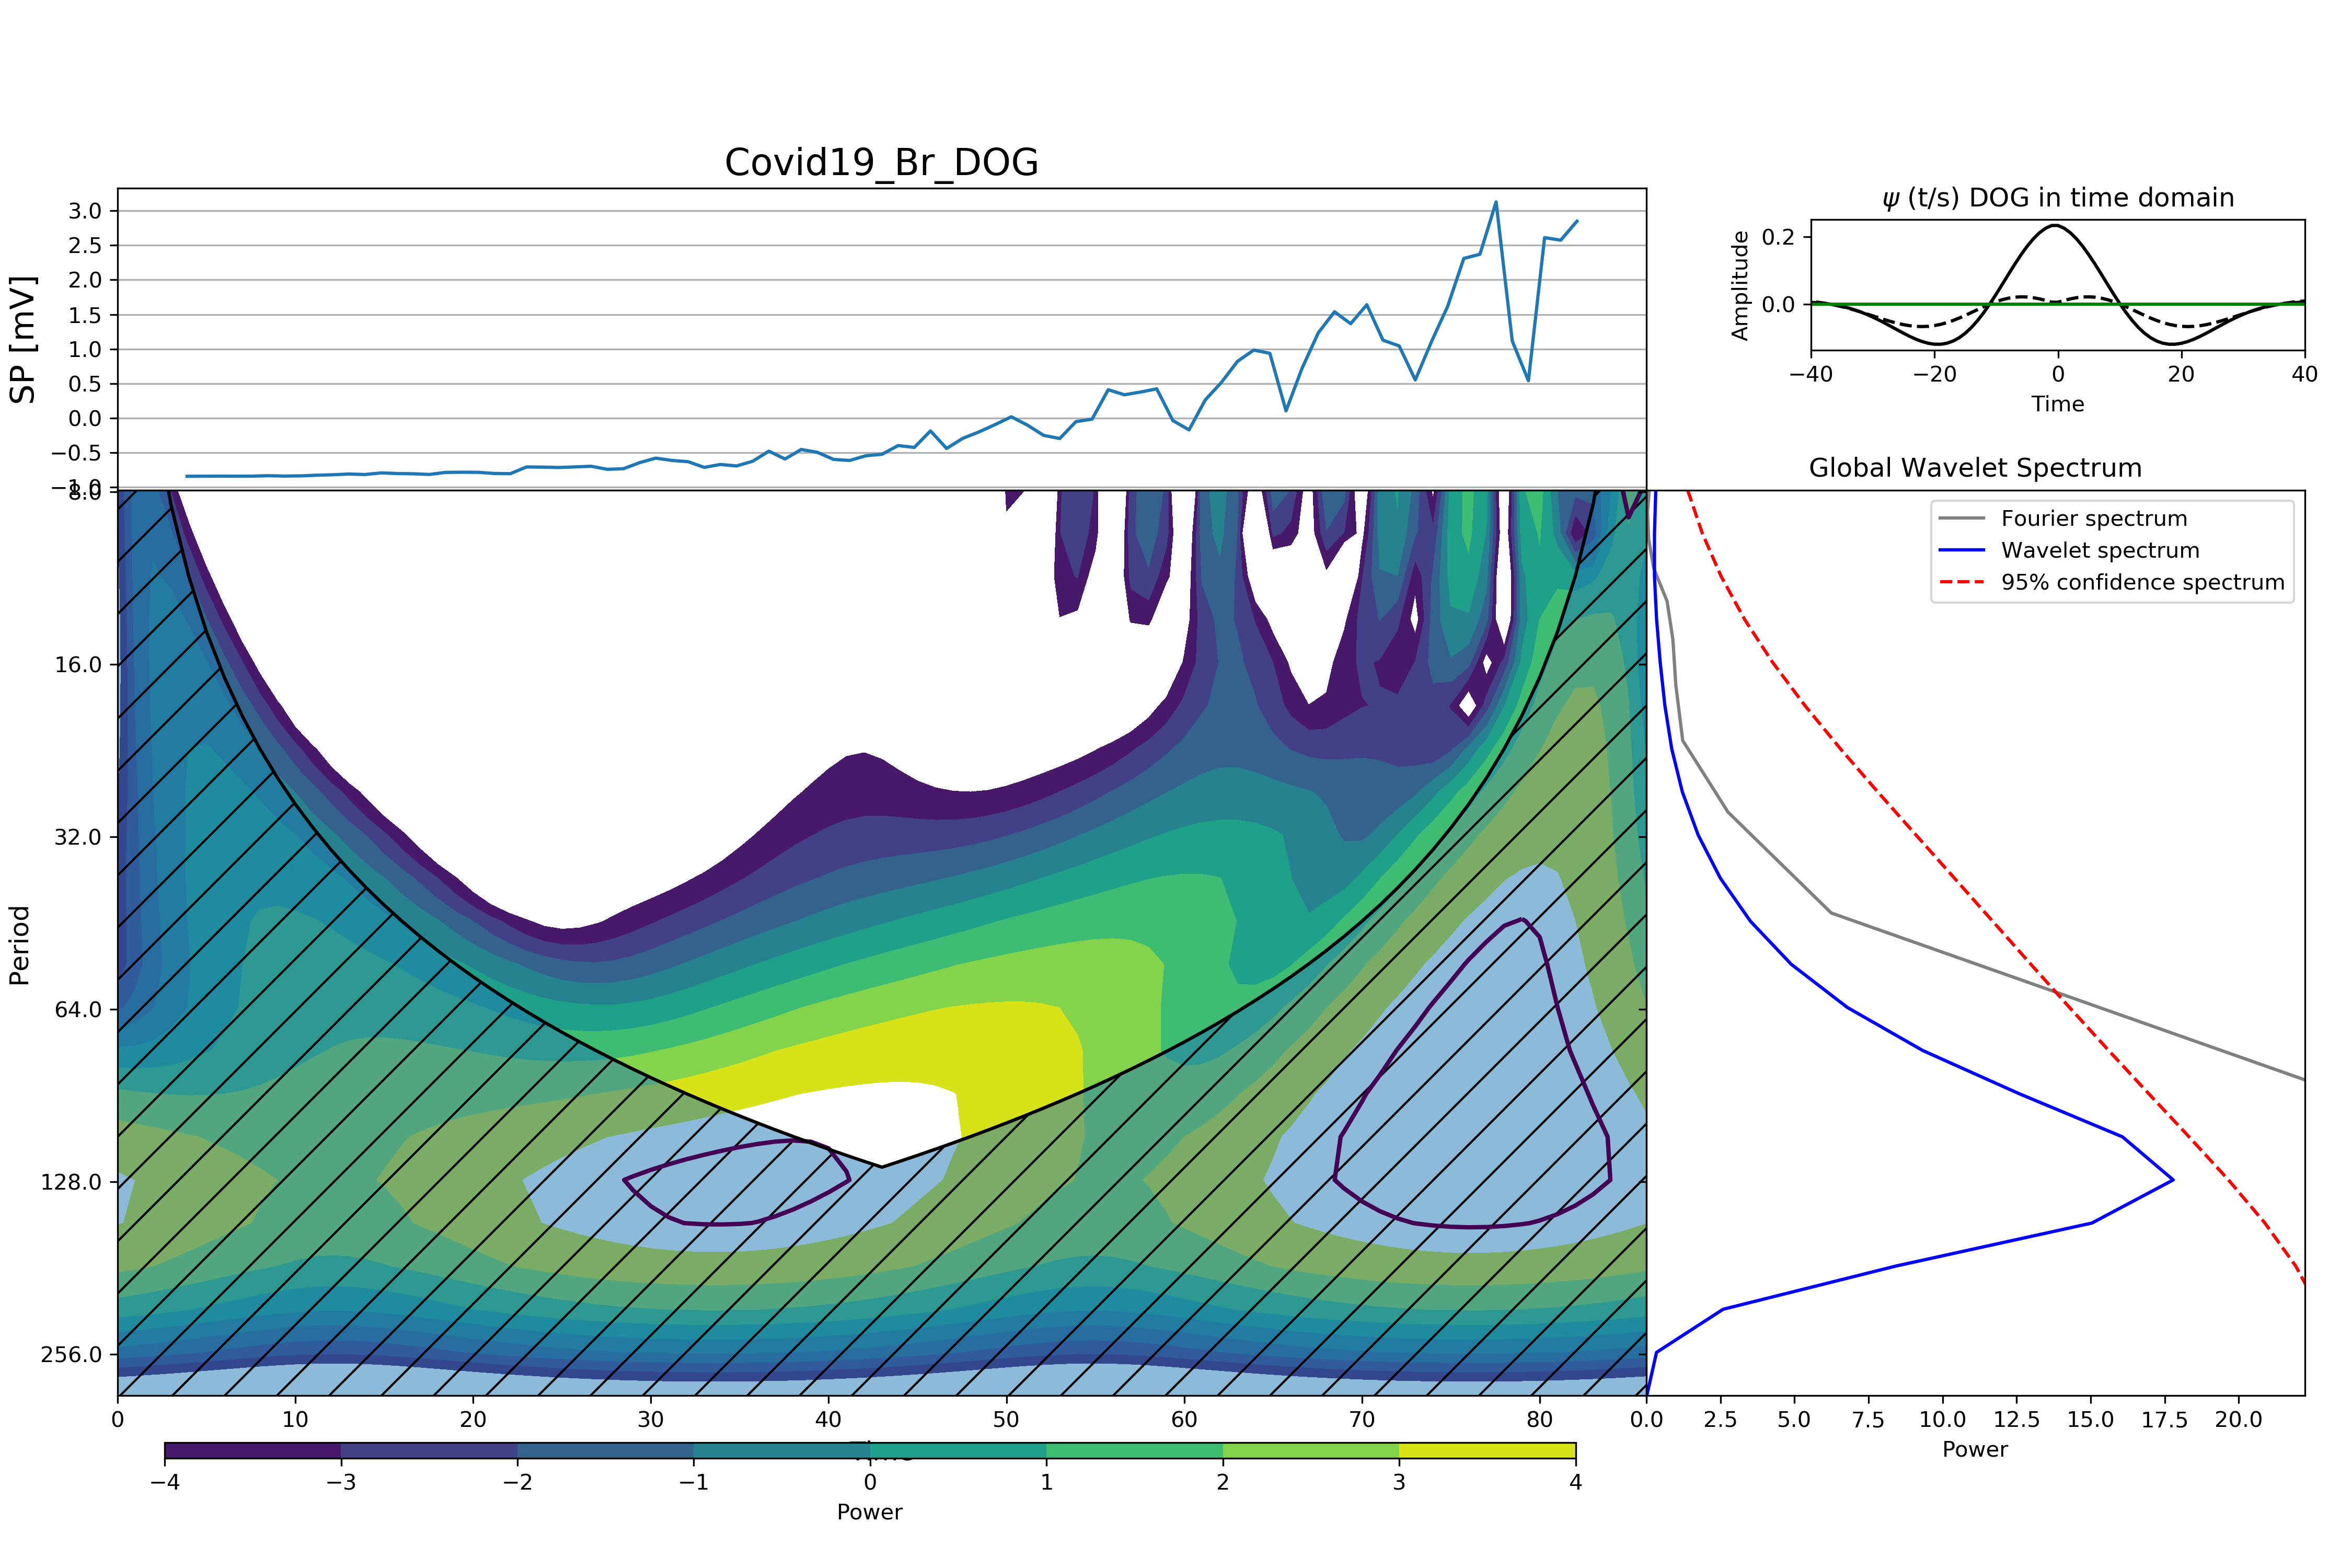
\includegraphics{Figuras/ex8/Covid19_Br_DOG.png}}		
	\end{center}
	\vspace{-2mm}	% acrescentar o espaçamento vertical apropriado entre a borda inferior da figura e a legenda ou a fonte quando não há legenda (o valor pode ser negativo para subir)
	\legenda{Figura 8.2.1: Global Wavelet Spectrum da série de dados da Covid19 do Brasil com a ondeleta mãe DoG (Derivative of Gaussian).}	% legenda - para deixar sem legenda usar comando \legenda{} (nunca deve-se comentar o comando \legenda)
	\label{ex8_fig1}
	%\FONTE{}	% fonte consultada (elemento obrigatório, mesmo que seja produção do próprio autor)
\end{figure}